\Subsection{Билет 62: Формула Грина. Формулы для вычисления площади.}

\begin{definition}\thmslashn
	
	$\Omega \subset \R^2$ элементарная область, если 
	
	$\Omega = \{ (x, y): x \in (a, b) $ и $ \phi(x) < y < \psi(x) \} = \{ (x, y): y \in (c, d) $ и $ \alpha(y) < x < \beta(y) \}$, 
	
	где $\alpha, \beta, \phi, \psi$ -- непрерывные функции
	
\end{definition}

\begin{theorem}[Формула Грина]\thmslashn
	
	$\Omega \subset \R^2$ ограниченная область, граница которой состоит из конечного числа попарно непересекающихся простых кусочко-гладких контуров, ориентированных положительно
	
	$\omega = P\,dx + Q\,dy$, где $P, Q, \frac{\partial P}{\partial y}, \frac{\partial Q}{\partial x}$ непрерывны на $\Cl \Omega$ (т.е. из можно доопределить на границе с сохранением непрерывности)
	
	Тогда $\int\limits_\Omega \left( \frac{\partial Q}{\partial x}-\frac{\partial P}{\partial y} \right) \,dx\,dy = \int\limits_{\partial \Omega} P\,dx + Q\,dy$
	
\end{theorem}

\begin{remark_author}\thmslashn

	$\partial \Omega$ -- граница области $\Omega$
	
	Ориентированных положительно -- ориентировать переход так, чтобы область была слева

\end{remark_author}

\begin{proof}\thmslashn
	
	Надо доказать 2 формулы $\int\limits_\Omega \frac{\partial P}{\partial y}\,dx\,dy = -\int\limits_{\partial \Omega} P\,dx$ и $\int\limits_\Omega \frac{\partial Q}{\partial x}\,dx\,dy = \int\limits_{\partial \Omega} Q\,dy$
	
	Заметим, что мы можем менять порядок интегрирования, тк все производные непрерывны на замыкании области. $\Omega$ -- ограниченная $\Rightarrow$ мы интегрируем непрерывную функцию по компактному множеству $\Rightarrow$ по теореме Фубини можем менять порядок.
	
	Проверим первую формулу
	
	\begin{enumerate}[Шаг 1.]

		\item
		$\Omega$ -- элементарная область 
		
		$\int\limits_\Omega \frac{\partial P}{\partial y}\,dy\,dx = \int\limits_a^b\int\limits_{\phi(x)}^{\psi(x)} \frac{\partial P}{\partial y}(x, y) \,dy\,dx = \int\limits_a^b P(x, \psi(x)) \,dx -\int\limits_a^b P(x, \phi(x)) \,dx$
		
		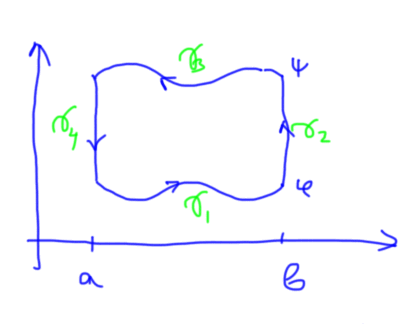
\includegraphics[scale=0.5]{pic_1}
		
		$\int\limits_\gamma P \,dx = \int\limits_{\gamma_1} + \int\limits_{\gamma_2} + \int\limits_{\gamma_3} + \int\limits_{\gamma_4}$
		
		$\int\limits_{\gamma_2} P\,dx= \int\limits_{\phi(x)}^{\psi(x)} P(b, t) \cdot b' \,dt = 0 = \int\limits_{\gamma_4} P\,dx$
		
		$\int\limits_{\gamma_1} P\,dx = \int\limits_{a}^{b} P(t, \phi(t)) \cdot t' \,dt$
		
		$\int\limits_{\gamma_3} P\,dx = \int\limits_{b}^{a} P(t, \psi(t)) \cdot t' \,dt$
		
		$\int\limits_a^b P(x, \psi(x)) \,dx -\int\limits_a^b P(x, \phi(x)) \,dx = -\int_{\gamma_3} P\,dx -\int_{\gamma_1} P\,dx = -\int\limits_\gamma P \,dx$

		\item
		Если ф-ла верна для двух областей, то она верна и для из определения. 
		
		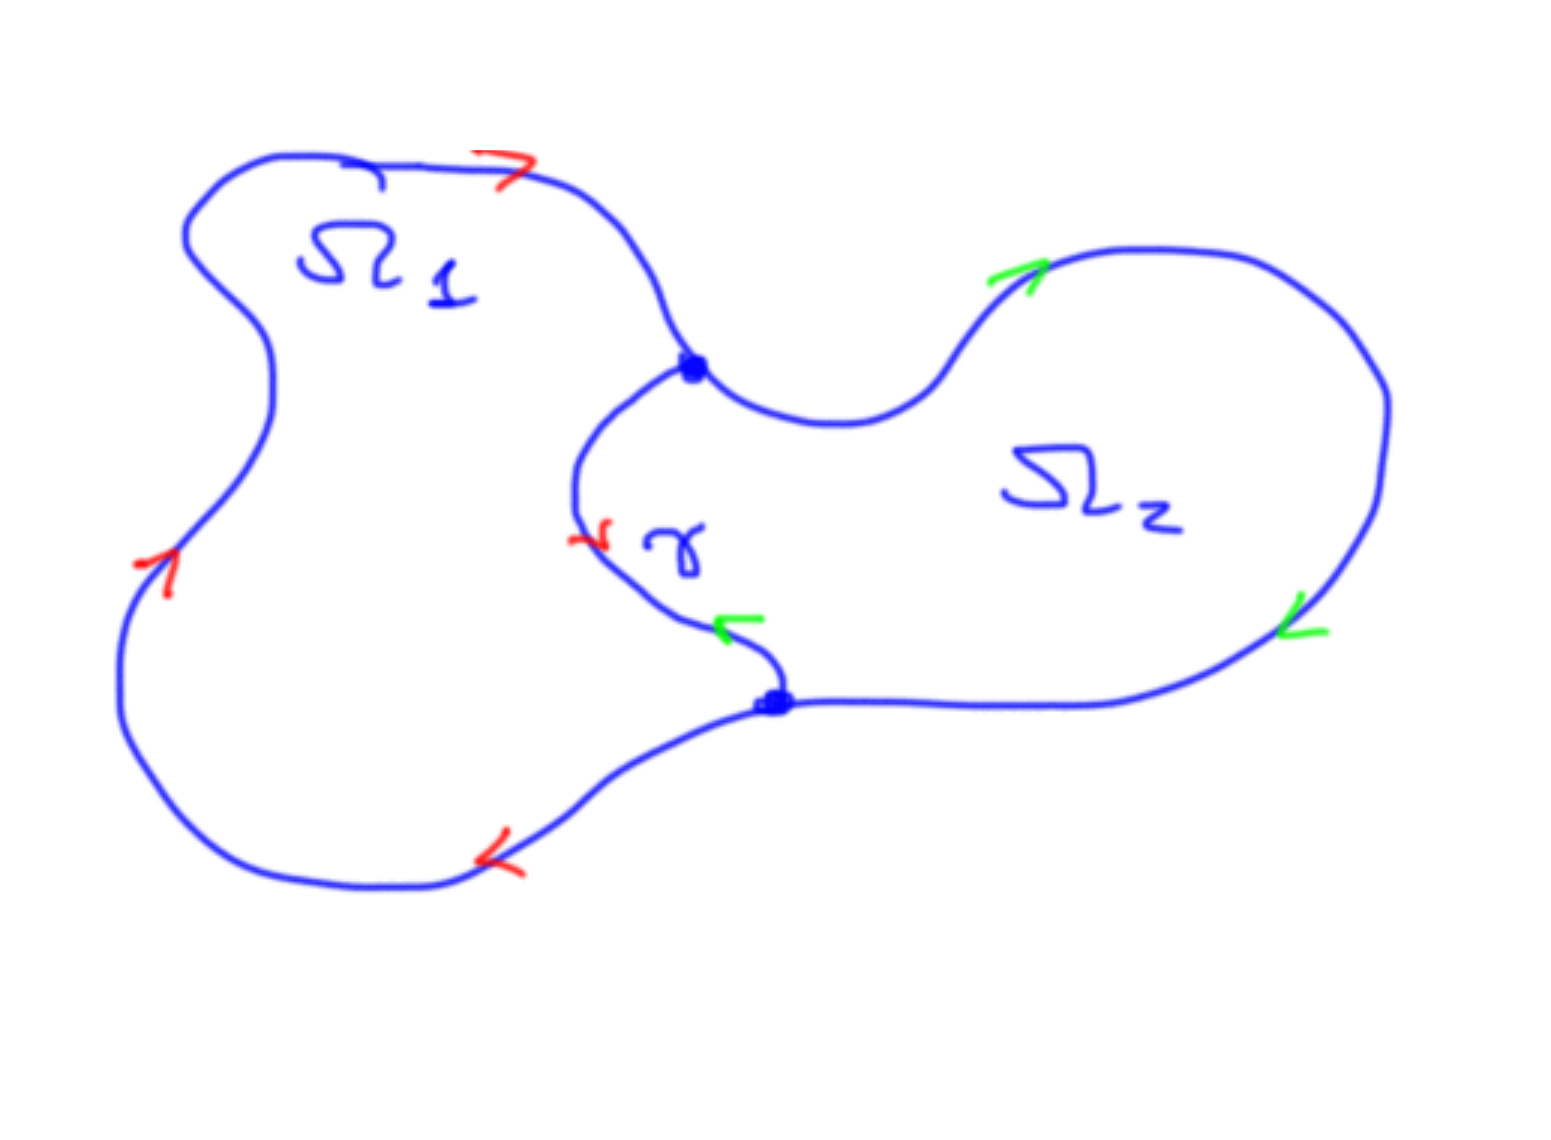
\includegraphics[scale=0.5]{pic_2}
		
		$\Omega = \Omega_1 \cup \Omega_2 \cup \gamma$
		
		$\int\limits_\Omega \frac{\partial P}{\partial y}\,dx\,dy = \int\limits_{\Omega_1} \frac{\partial P}{\partial y}\,dx\,dy + \int\limits_{\Omega_2} \frac{\partial P}{\partial y}\,dx\,dy = -\int\limits_{\partial \Omega_1} P \,dx -\int\limits_{\partial \Omega_2} P \,dx = -\int\limits_{\partial \Omega} P \,dx - \int\limits_{\gamma} P \,dx - \int\limits_{-\gamma} P \,dx = -\int\limits_{\partial \Omega} P \,dx $

		\item
		Формула верна для конечного объединения элем. областей
		
		\item
		Любая область из условия теоремы может быть разрезана на конечное число элементарных областей
		
		(д-ть не будем)

	\end{enumerate}
\end{proof}

\begin{consequence}\thmslashn

	$\lambda_2 \Omega = \int\limits_{\partial \Omega} x \,dy = - \int\limits_{\partial \Omega} y \,dx = \frac{1}{2} \int\limits_{\partial \Omega} x \,dy - y \,dx $

\end{consequence}

\begin{proof}\thmslashn

	$P = 0,\;\; Q = x \Rightarrow   \frac{\partial Q}{\partial x} - \frac{\partial P}{\partial y} = 1$
	
	Подставляем в формулу Грина
	
	$\int\limits_{\partial \Omega} x \,dy = \int\limits_{\partial \Omega} P \,dx + Q\,dy = \int\limits_{\Omega} \left(  \frac{\partial Q}{\partial x}-\frac{\partial P}{\partial y} \right) \, d\lambda_2 =  \int\limits_{\Omega} 1 \,d\lambda_2 = \lambda_2 \Omega$
	
	И теперь в другую сторону
	
	$P = -\frac{y}{2},\;\; Q = \frac{x}{2} \Rightarrow   \frac{\partial Q}{\partial x} - \frac{\partial P}{\partial y} = 1$

\end{proof}

\begin{remark}\thmslashn
	
	$\gamma(t) = (x(t), y(t)),\;\; \gamma : [a, b] \to \R$
	
	$\int\limits_{\gamma} x \,dy = \int\limits_a^b x(t)y'(t)\,dt$
	
	$-\int\limits_{\gamma} y \,dx = -\int\limits_a^b y(t)x'(t)\,dt$
	
\end{remark}